% Provenance (never printed): enseignement scientifique premiere (2019),
% theme "La Terre, un astre singulier: la forme de la Terre" (Eratosthenes,
% meridian measurement by triangulation, the metre); see
% sources/book2/PROVENANCE.md. Every length on the ellipsoid is computed in
% figdata/grade-10/meridian_degree.py (WGS 84, ledger wgs84:ellipsoid).
\chapter{Mesurer la Terre}\label{ch:g10:measuring-the-earth}

Sur une plage, regardons un navire s'éloigner vers le large. Il ne se
contente pas de rapetisser jusqu'à devenir invisible~: sa coque disparaît
d'abord, comme s'il sombrait, puis le bas de ses superstructures, et le
sommet de son mât en dernier. La mer qui nous sépare du navire n'est pas
plane~: elle est bombée. Il y a plus de vingt-deux siècles, un savant
d'Alexandrie a tiré d'une observation du même genre --- la longueur d'une
ombre à midi --- la mesure de la taille de la planète entière. Ce chapitre
suit cette mesure et celles qui l'ont suivie~: les chaînes de triangles que
les arpenteurs ont tendues à travers des pays entiers, les expéditions
envoyées dans l'Arctique et à l'équateur pour savoir si la Terre est aplatie,
la naissance du mètre, et les satellites avec lesquels on mesure aujourd'hui
la planète.

\begin{omfigure}
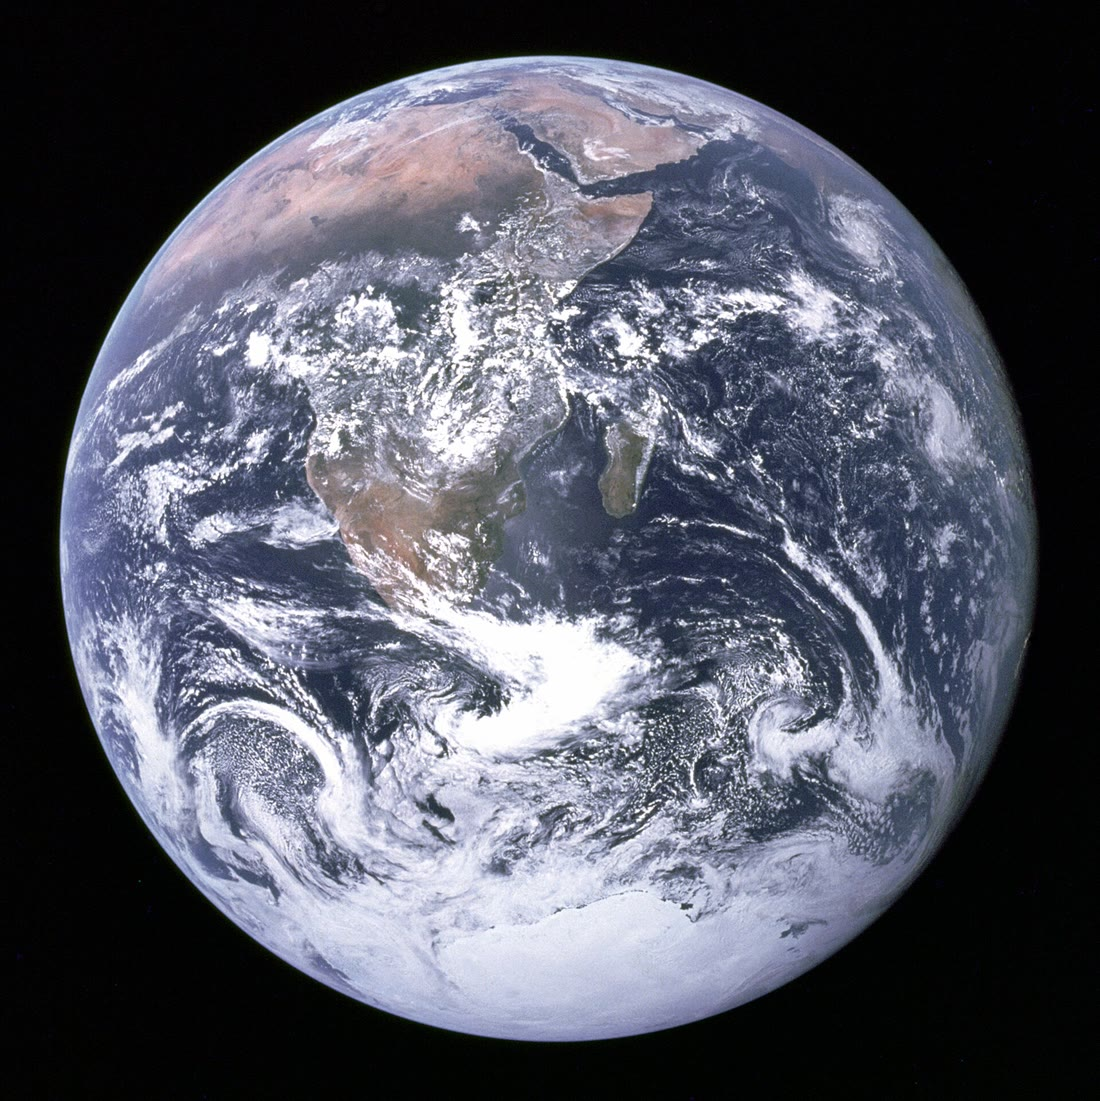
\includegraphics[width=0.5\linewidth]{images/book2/g10-nasa-apollo17-earth.jpg}

{\small La Terre photographiée par l'équipage d'Apollo~17 en route vers la
Lune, en décembre 1972~: l'Afrique, l'Arabie et les glaces de l'Antarctique.
Photographie~: NASA (domaine public).}
\end{omfigure}

\begin{recall}
Un lieu de la Terre est repéré par sa latitude, son angle au nord ou au sud
de l'équateur, et par sa longitude, son angle à l'est ou à l'ouest d'un
méridien de référence~; les méridiens joignent les pôles, les parallèles
font le tour de la Terre parallèlement à l'équateur (livre~1). Dans un
milieu homogène, la lumière se propage en ligne droite, et les rayons qui
nous arrivent du Soleil, très lointain, sont parallèles (les livres de
physique). Dans un triangle rectangle, le sinus d'un angle aigu est le côté
opposé divisé par l'hypoténuse, son cosinus le côté adjacent divisé par
l'hypoténuse, sa tangente le côté opposé divisé par le côté adjacent (les
livres de mathématiques).
\end{recall}

\section{Une Terre ronde}

Bien avant que quiconque puisse regarder la Terre depuis l'espace, plusieurs
observations montraient qu'elle est ronde.
\begin{itemize}
  \item \textbf{Les navires sous l'horizon.} Un navire qui s'éloigne
        disparaît par le bas, dans toutes les directions et sur toutes les
        mers~: la surface de la mer est partout courbe.
  \item \textbf{L'ombre sur la Lune.} Lors d'une éclipse de Lune, l'ombre de
        la Terre tombe sur la Lune. Son bord est toujours un arc de cercle,
        quelle que soit l'heure de la nuit~; seule une sphère projette une
        ombre ronde dans toutes les directions.
  \item \textbf{Les étoiles changent avec la latitude.} Un voyageur qui va
        vers le nord voit l'étoile Polaire monter au-dessus de l'horizon,
        et des étoiles du ciel austral disparaître sous lui~: l'horizon du
        voyageur s'incline à mesure qu'il se déplace sur une surface courbe.
  \item \textbf{Le tour du monde et la vue depuis l'espace.} Des navires,
        puis des avions, ont fait le tour du monde dans toutes les
        directions~; depuis les années 1960, on photographie la planète
        entière, bien ronde.
\end{itemize}

\begin{omfigure}
\begin{tikzpicture}[font=\small, >={Stealth[length=2.2mm]}]
  % sea surface: arc of a circle of radius 8 centred at (0,-8) (curvature exaggerated)
  \fill[omDef!10] plot[domain=-4.6:4.6, samples=60] (\x,{sqrt(64-\x*\x)-8}) -- (4.6,-2.2) -- (-4.6,-2.2) -- cycle;
  \draw[omDef!70!black, thick] plot[domain=-4.6:4.6, samples=60] (\x,{sqrt(64-\x*\x)-8});
  % observer on a small tower at x=-4 (surface y=-1.072), eye at y=-0.235
  \draw[black!70, line width=1pt] (-4,-1.072) -- (-4,-0.235);
  \fill (-4,-0.235) circle (2pt);
  \node[anchor=east, align=right] at (-4.1,-0.2) {œil de\\l'observateur};
  % line of sight tangent at x=-0.5 (y=-0.0156, slope 0.0626)
  \draw[omThm!80!black, thick] (-4,-0.235) -- (4.4,0.290);
  \node[omThm!80!black, anchor=south, rotate=3.6] at (1.3,0.1) {ligne de visée};
  \fill[omThm!80!black] (-0.5,-0.0156) circle (1.4pt);
  % ship at x=3 (surface y=-0.584), tilted 22 degrees with the local vertical
  \begin{scope}[shift={(3,-0.584)}, rotate=-22]
    \fill[black!12] (-0.6,0) -- (0.6,0) -- (0.75,0.32) -- (-0.75,0.32) -- cycle;
    \draw[black!45, densely dashed] (-0.6,0) -- (0.6,0) -- (0.75,0.32) -- (-0.75,0.32) -- cycle;
    \draw[black!45, densely dashed] (0,0.32) -- (0,0.95);
    \draw[black!80, line width=1pt] (0,0.95) -- (0,1.55);
    \fill[black!80] (0,1.55) -- (0.32,1.25) -- (0,1.25) -- cycle;
  \end{scope}
  \node[anchor=north, align=center, font=\footnotesize] at (2.9,-1.25) {coque et bas du mât\\cachés par le bombement};
  \node[anchor=north, font=\footnotesize] at (-0.5,-0.1) {horizon};
\end{tikzpicture}

{\small Pourquoi un navire disparaît par le bas~: l'observateur ne voit que
ce qui se trouve au-dessus de la ligne de visée qui frôle la mer à
l'horizon. La courbure est très exagérée.}
\end{omfigure}

\section{Ératosthène mesure la Terre}

Ératosthène de Cyrène (276--194 av. J.-C.) était le bibliothécaire
d'Alexandrie. Il avait appris qu'à Syène, l'actuelle Assouan, loin en amont
sur le Nil, le Soleil éclairait à midi tout le fond d'un puits le jour du
solstice d'été~: il était alors exactement au zénith. À Alexandrie, au même
moment, un bâton vertical projetait une ombre courte~: les rayons du Soleil
faisaient avec la verticale un angle d'environ \qty{7.2}{\degree}, un
cinquantième de tour complet.
% ledger: erat:method, erat:stadion

\begin{omfigure}
\begin{tikzpicture}[font=\small, >={Stealth[length=2.2mm]}]
  \def\R{2.4}
  \fill[omDef!8] (0,0) circle (\R);
  \draw[omDef!70!black, thick] (0,0) circle (\R);
  \coordinate (O) at (0,0);
  \coordinate (S) at (\R,0);
  \coordinate (A) at ({\R*cos(25)},{\R*sin(25)});
  \coordinate (T) at ({(\R+0.75)*cos(25)},{(\R+0.75)*sin(25)});
  \coordinate (T2) at ({(\R+1.75)*cos(25)},{(\R+1.75)*sin(25)});
  % radii
  \draw[black!70] (O) -- (S);
  \draw[black!70] (O) -- (A);
  \draw[black!40, densely dashed] (A) -- (T2);
  \fill (O) circle (1.5pt) node[below left] {centre};
  % stick at Alexandria, along the radius
  \draw[line width=1.6pt, black!85] (A) -- ($(A)!0.6!(T)$);
  % well at Syene
  \draw[black!80, thick] ({\R-0.38},-0.12) -- (\R,-0.12) ($(S)+(0,0.12)$) -- ({\R-0.38},0.12);
  % parallel sun rays coming from the right
  \foreach \y in {-1.6,-0.8,0.8,1.6} \draw[->, omThm!70, thick] (6.6,\y) -- (4.4,\y);
  \draw[->, omThm!85!black, thick] (6.6,0) -- (\R+0.05,0);
  \draw[->, omThm!85!black, thick] (6.6,{(\R+0.45)*sin(25)}) -- ({(\R+0.45)*cos(25)+0.03},{(\R+0.45)*sin(25)});
  \node[omThm!85!black, align=center, anchor=west] at (4.6,2.35) {lumière solaire~:\\rayons parallèles};
  % angles
  \draw[omExo!80!black, thick] (0.75,0) arc (0:25:0.75);
  \node[omExo!80!black] at (1.05,0.22) {$\alpha$};
  \coordinate (Q) at ($(A)!0.6!(T)$);
  \draw[omExo!80!black, thick] ($(Q)+(0.8,0)$) arc (0:25:0.8);
  \node[omExo!80!black] at ($(Q)+({1.08*cos(12.5)},{1.08*sin(12.5)})$) {$\alpha$};
  \node[anchor=east] at ($(A)+(-0.12,0.18)$) {Alexandrie};
  \node[anchor=north west] at ($(S)+(0.3,-0.12)$) {Syène};
  \node[font=\footnotesize, anchor=north] at ($(O)!0.5!(S)+(0.2,-0.05)$) {};
  \draw[<->, black!60] ({(\R-0.3)*cos(3)},{(\R-0.3)*sin(3)}) arc (3:22:{\R-0.3});
  \node[anchor=east, font=\footnotesize] at ({(\R-0.35)*cos(13)},{(\R-0.35)*sin(13)}) {$d$};
\end{tikzpicture}

{\small Le raisonnement d'Ératosthène. À Syène, le Soleil est au zénith~: ses
rayons sont dirigés vers le centre de la Terre. À Alexandrie, un bâton
vertical, lui aussi dirigé vers le centre, fait un angle $\alpha$ avec les
rayons. L'angle au centre entre les deux lieux est ce même $\alpha$.
L'angle est exagéré~: il ne valait que \qty{7.2}{\degree}.}
\end{omfigure}

\begin{proposition}[La relation d'Ératosthène]\label{prop:g10:measuring-the-earth:eratosthenes}
Si deux lieux sont situés sur le même méridien, à une distance $d$ l'un de
l'autre, et si les rayons du Soleil à midi font avec la verticale des angles
qui diffèrent de $\alpha$ (en degrés), la circonférence de la Terre vaut
\[
  C = \frac{\qty{360}{\degree}}{\alpha}\, d .
\]
\end{proposition}

\begin{proof}
Le Soleil est si loin que ses rayons qui atteignent les deux lieux sont
parallèles. En chaque lieu, la verticale est dirigée vers le centre de la
Terre. Sur la figure, le rayon qui atteint le bâton et le rayon terrestre
passant par Syène sont deux droites parallèles, et le rayon terrestre
passant par Alexandrie les coupe toutes deux~: l'angle $\alpha$ entre le
bâton et le rayon lumineux et l'angle au centre entre les deux rayons
terrestres sont alternes-internes, donc égaux. L'arc $d$ représente la même
fraction de la circonférence entière que l'angle $\alpha$ d'un tour
complet~: $d/C = \alpha/\qty{360}{\degree}$.
\end{proof}

\begin{method}[Mesurer une circonférence à partir de deux ombres]\label{met:g10:measuring-the-earth:shadows}
\begin{enumerate}
  \item Choisir deux lieux situés (presque) sur le même méridien et mesurer
        la distance nord--sud $d$ qui les sépare.
  \item Le même jour, au midi local, mesurer en chaque lieu l'angle entre un
        bâton vertical et les rayons du Soleil~: $\tan \theta = s/h$, où $h$
        est la hauteur du bâton et $s$ la longueur de son ombre. Ne jamais
        regarder le Soleil lui-même~: l'angle se lit sur l'ombre seule.
  \item Faire la différence $\alpha$ des deux angles et appliquer
        $C = (360/\alpha)\,d$.
\end{enumerate}
\end{method}

\begin{example}[Les nombres d'Ératosthène]\label{ex:g10:measuring-the-earth:numbers}
% ledger: erat:method, erat:stadion
Ératosthène prenait pour distance d'Alexandrie à Syène 5000
\emph{stades}, une unité de longueur grecque. Avec $\alpha = 1/50$ de tour,
\[
  C = 50 \times 5000 = 250\,000 \text{ stades}.
\]
Que valait un stade~? Les historiens en débattent encore. Avec
\qty{157.2}{m}, $C \approx \qty{39300}{km}$~; avec \qty{166.7}{m},
$C \approx \qty{41700}{km}$. La vraie circonférence méridienne est de
\qty{40008}{km}~: dans les deux cas, Ératosthène était à quelques pour cent
près.
\end{example}

\begin{remark}[Les hypothèses]\label{rem:g10:measuring-the-earth:assumptions}
Ératosthène supposait une Terre sphérique, un Soleil assez lointain pour
que ses rayons soient parallèles, Syène exactement sur le tropique (où le
Soleil peut passer au zénith) et Syène plein sud d'Alexandrie. Chacune de
ces hypothèses était presque vraie, mais pas tout à fait~: Assouan est
située à environ \qty{3}{\degree} de longitude à l'est d'Alexandrie. Ce qui
compte est la composante nord--sud de la distance, celle qui suit le
méridien.
% ledger: geonames:aswan, geonames:alexandria
\end{remark}

\section{La triangulation}

Mesurer une longue distance au sol avec une chaîne ou une règle est lent,
et impossible à travers les fleuves, les forêts et les montagnes. Les
angles, en revanche, se mesurent très précisément avec une lunette montée
sur un cercle gradué, pointée tour à tour vers deux signaux lointains. À
partir du \textsc{xviii}\textsuperscript{e}~siècle, les géomètres s'en sont
servis pour mesurer des pays entiers.

\begin{definition}[Géodésie]\label{def:g10:measuring-the-earth:geodesy}
La \emph{géodésie}\index{geodesie@géodésie} est la science qui mesure la
forme et les dimensions de la Terre ainsi que la position des points de sa
surface, et qui suit leurs variations au cours du temps.
\end{definition}

\begin{definition}[Triangulation]\label{def:g10:measuring-the-earth:triangulation}
La \emph{triangulation}\index{triangulation} repère des points éloignés par
une chaîne de triangles~: un côté, la \emph{base}, est mesuré au sol avec un
très grand soin~; tous les angles des triangles sont mesurés depuis leurs
sommets~; tous les autres côtés sont ensuite calculés.
\end{definition}

Le calcul repose sur une relation entre les côtés et les angles d'un
triangle quelconque. Dans un triangle $ABC$, notons $a$, $b$, $c$ les côtés
opposés aux sommets $A$, $B$, $C$, et $A$, $B$, $C$ aussi les angles en ces
sommets.

\begin{proposition}[La loi des sinus]\label{prop:g10:measuring-the-earth:sine-rule}
Dans tout triangle $ABC$,
\[
  \frac{a}{\sin A} = \frac{b}{\sin B} = \frac{c}{\sin C}.
\]
\end{proposition}

\begin{proof}
Traçons la hauteur issue de $C$, qui coupe la droite $AB$ en $H$ (second
panneau de la figure ci-dessous)~; notons $h = CH$. Dans le triangle
rectangle $AHC$, $\sin A = h/b$, donc $h = b \sin A$. Dans le triangle
rectangle $BHC$, $\sin B = h/a$, donc $h = a \sin B$. Ainsi
$b \sin A = a \sin B$, c'est-à-dire $a/\sin A = b/\sin B$. (Si l'angle en
$B$ est obtus, $H$ tombe au-delà de $B$ et l'angle du triangle rectangle
en $B$ vaut $\qty{180}{\degree} - B$, qui a le même sinus.) Le même
raisonnement avec la hauteur issue de $A$ donne $b/\sin B = c/\sin C$.
\end{proof}

\begin{omfigure}
\begin{tikzpicture}[font=\small, >={Stealth[length=2mm]}]
  \begin{scope}
    \coordinate (A) at (0,0); \coordinate (B) at (2.0,0.25);
    \coordinate (C) at (0.9,1.9); \coordinate (D) at (3.0,2.1);
    \coordinate (E) at (1.9,3.8); \coordinate (F) at (3.9,4.1);
    \coordinate (G) at (2.7,5.6);
    \draw[black!60] (A) -- (C) -- (B) (C) -- (D) -- (B) (C) -- (E) -- (D) -- (F) -- (E) -- (G) -- (F);
    \draw[omThm!85!black, line width=2pt] (A) -- (B);
    \foreach \p in {A,B,C,D,E,F,G} \fill (\p) circle (1.6pt);
    \node[below left] at (A) {$A$}; \node[below right] at (B) {$B$};
    \node[left] at (C) {$C$}; \node[right] at (D) {$D$};
    \node[left] at (E) {$E$}; \node[right] at (F) {$F$}; \node[above] at (G) {$G$};
    \node[omThm!85!black, anchor=north, font=\footnotesize] at (1.25,-0.3) {base mesurée};
    \draw[omExo!80!black] ($(A)!0.28!(B)$) arc[start angle=7, end angle=64.6, radius=0.56];
    \draw[omExo!80!black] ($(B)!0.3!(A)$) arc[start angle=187, end angle=123, radius=0.6];
    \draw[black!50, densely dashed] (-0.5,0) -- (-0.5,5.6);
    \draw[->, black!70] (-0.5,5.0) -- (-0.5,5.8) node[above] {N};
    \node[rotate=90, font=\footnotesize, black!60, anchor=south] at (-0.5,2.6) {méridien};
  \end{scope}
  \begin{scope}[xshift=6.2cm, yshift=0.6cm]
    \coordinate (A) at (0,0); \coordinate (B) at (4,0); \coordinate (C) at (1.4,2.6);
    \coordinate (H) at (1.4,0);
    \draw[thick] (A) -- (B) -- (C) -- cycle;
    \draw[omDef!80!black, densely dashed] (C) -- (H);
    \draw[omDef!80!black] (1.4,0.22) -- (1.62,0.22) -- (1.62,0);
    \node[below left] at (A) {$A$}; \node[below right] at (B) {$B$};
    \node[above] at (C) {$C$}; \node[below] at (H) {$H$};
    \node[omDef!80!black, anchor=west] at (1.4,1.05) {$h$};
    \node[anchor=south east] at (0.7,1.3) {$b$};
    \node[anchor=south west] at (2.75,1.35) {$a$};
    \node[anchor=north] at (2.7,-0.02) {$c$};
    \draw[omExo!80!black] (0.5,0) arc (0:61.7:0.5);
    \draw[omExo!80!black] (3.45,0) arc (180:135:0.55);
  \end{scope}
\end{tikzpicture}

{\small À gauche~: une chaîne de triangles tendue le long d'un méridien à
partir d'une base mesurée $AB$~; les arcs marquent deux des nombreux angles
mesurés avec l'instrument. À droite~: la hauteur $h$ issue de $C$, écrite de
deux façons, donne la loi des sinus.}
\end{omfigure}

\begin{method}[Calculer une chaîne de triangulation]\label{met:g10:measuring-the-earth:chain}
\begin{enumerate}
  \item Dans le premier triangle $ABC$, on mesure la base $c = AB$ et les
        angles en $A$ et en $B$~; le troisième angle vaut
        $C = \qty{180}{\degree} - A - B$ (et sa mesure contrôle les
        autres).
  \item La loi des sinus donne les deux autres côtés~:
        $b = AC = c \sin B / \sin C$ et $a = BC = c \sin A / \sin C$.
  \item Un côté calculé devient le côté connu du triangle suivant, et ainsi
        de suite le long de la chaîne.
  \item Enfin, on calcule la composante nord--sud de chaque côté avec le
        cosinus de son angle avec le méridien, et on additionne ces
        composantes.
\end{enumerate}
\end{method}

\begin{example}[Un triangle]\label{ex:g10:measuring-the-earth:triangle}
On mesure une base $AB = \qty{8.000}{km}$~; depuis $A$, le signal $C$ est
vu à \qty{70}{\degree} de la direction de $B$, depuis $B$ à
\qty{60}{\degree} de la direction de $A$. Alors $C = \qty{50}{\degree}$ et
\[
  AC = \frac{8.000 \times \sin 60^\circ}{\sin 50^\circ} = \frac{8.000 \times 0.8660}{0.7660}
  \approx \qty{9.044}{km}, \qquad
  BC = \frac{8.000 \times \sin 70^\circ}{\sin 50^\circ} \approx \qty{9.814}{km}.
\]
Seule la base a été parcourue à pied.
\end{example}

\begin{example}[Le méridien du mètre]\label{ex:g10:measuring-the-earth:meridian}
% ledger: metre:1791, metre:survey, geonames:dunkirk, geonames:barcelona (arc computed in figdata/grade-10/meridian_degree.py)
En mars 1791, le mètre fut défini comme la dix-millionième partie de la
distance du pôle à l'équateur le long d'un méridien. Pour connaître cette
distance, deux astronomes, Jean-Baptiste Delambre et Pierre Méchain,
mesurèrent par \omterm{def:g10:measuring-the-earth:triangulation}{triangulation} l'arc de méridien de Dunkerque, sur la mer du
Nord, à Barcelone, sur la Méditerranée --- près de sept ans de travail,
Delambre dans les deux tiers nord, Méchain dans le tiers sud. Les deux
villes diffèrent de \qty{9.646}{\degree} de latitude~; sur l'ellipsoïde
moderne, l'arc compris entre leurs parallèles mesure \qty{1072.2}{km}.
Connaître la longueur d'un arc et sa différence de latitude donne la
longueur d'un degré~; la forme de la Terre donne ensuite le quart de
méridien entier. Des étalons en platine du nouveau mètre furent réalisés en
1799 et déposés aux Archives nationales.
\end{example}

\begin{history}[Le cercle répétiteur]
Les angles du méridien du mètre furent mesurés avec un \emph{cercle
répétiteur}, un instrument construit par Jean-Charles de Borda~: deux
lunettes montées sur un cercle gradué, pointées alternativement vers deux
signaux un grand nombre de fois, si bien que les erreurs de lecture de la
graduation sont divisées par le nombre de répétitions.
\begin{center}
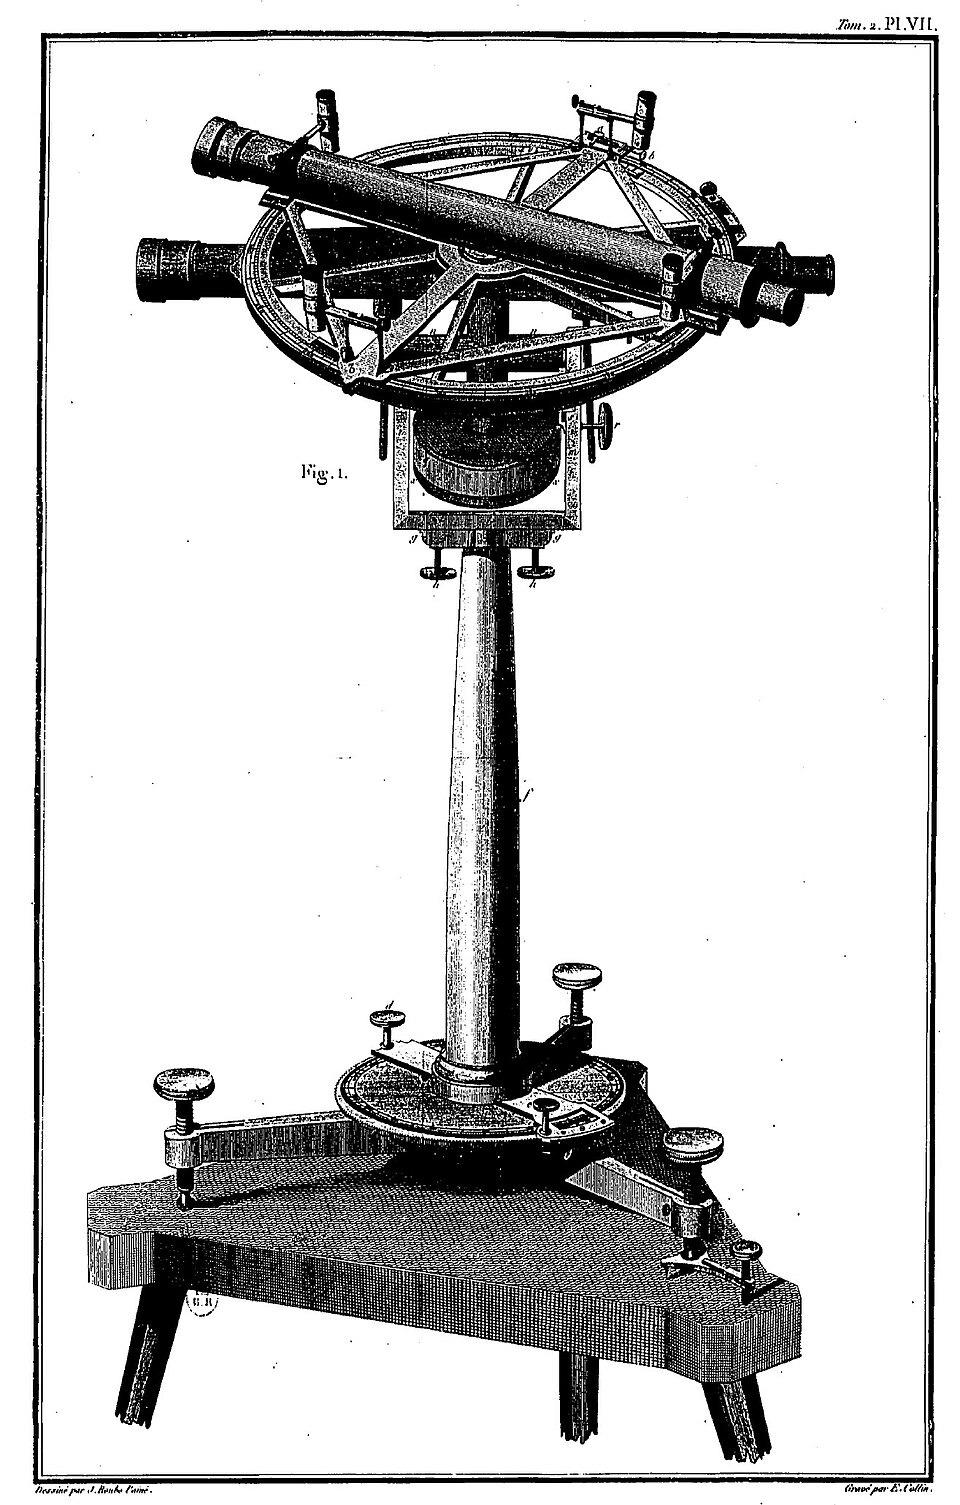
\includegraphics[width=0.3\linewidth]{images/book2/g10-delambre-repeating-circle.jpg}

{\small Un cercle répétiteur monté pour mesurer des angles horizontaux, tel
qu'il est gravé dans le compte rendu de la mesure par Delambre (1807).
Domaine public (Wikimedia Commons).}
\end{center}
\end{history}

\section{Une Terre aplatie}

Vers 1687, Isaac Newton déduisit de sa théorie de la gravitation qu'une
Terre en rotation doit être un sphéroïde aplati aux pôles et renflé à
l'équateur. Les mesures de degrés du méridien faites par les astronomes de
l'Observatoire de Paris semblaient dire le contraire~: une Terre allongée
aux pôles. La question fut tranchée en mesurant la longueur d'un degré de
latitude en deux lieux aussi éloignés que possible.
% ledger: figure:expeditions

\begin{omfigure}
\begin{tikzpicture}[font=\small, >={Stealth[length=2mm]}]
  \def\a{3.0} \def\b{2.3}
  \draw[black!35, densely dashed] (0,0) circle (\a);
  \fill[omDef!8] (0,0) ellipse ({\a} and {\b});
  \draw[omDef!70!black, thick] (0,0) ellipse ({\a} and {\b});
  \draw[black!50] (-3.4,0) -- (3.7,0);
  \draw[black!50] (0,-2.6) -- (0,3.3);
  \draw[<->, omThm!85!black] (0,-0.3) -- (\a,-0.3);
  \node[omThm!85!black, below] at (1.5,-0.3) {$a$};
  \draw[<->, omThm!85!black] (-0.3,0) -- (-0.3,\b);
  \node[omThm!85!black, left] at (-0.3,1.15) {$b$};
  \node[above right] at (0,\b) {N};
  \node[anchor=south east] at (3.0,-2.5) {};
  \node[anchor=west] at (3.7,0) {équateur};
  % normal at t = 45 deg: P = (2.121, 1.626); crosses the equator at (0.874,0), the axis at (0,-1.14)
  \coordinate (P) at (2.121,1.626);
  \draw[omExo!85!black, thick] (P) -- ($(P)!1.35!(0.874,0)$);
  \draw[omExo!85!black, thick, ->] (P) -- ($(P)!-0.45!(0.874,0)$);
  \fill (P) circle (1.6pt);
  \node[anchor=west, align=left, font=\footnotesize] at (2.85,2.35) {verticale locale\\(fil à plomb)};
  \draw[omExo!85!black] (1.45,0) arc (0:52.5:0.58);
  \node[omExo!85!black] at (1.62,0.32) {$\varphi$};
  \fill (0,0) circle (1.3pt);
  \node[anchor=north east, font=\footnotesize] at (0,0) {centre};
  \node[black!50, font=\footnotesize, anchor=south] at (-2.2,2.15) {sphère};
\end{tikzpicture}

{\small Une Terre aplatie, avec un \omterm{def:g10:measuring-the-earth:ellipsoid}{aplatissement} très exagéré (le vrai est
trop faible pour être visible à cette échelle). La verticale d'un lieu est
perpendiculaire à la surface~; elle n'est pas dirigée exactement vers le
centre. La latitude $\varphi$ du lieu est l'angle entre sa verticale et le
plan de l'équateur.}
\end{omfigure}

La latitude se mesure à l'aide des étoiles~: c'est l'angle entre la
verticale locale et le plan de l'équateur. Sur une Terre aplatie, la surface
est moins courbe près des pôles que près de l'équateur. Là où la surface est
moins courbe, il faut la parcourir plus longtemps pour que la verticale
tourne d'un degré~: \emph{un degré de latitude est plus long près des pôles}.

\begin{history}[Laponie et Pérou]
% ledger: figure:expeditions, figure:degrees
En 1735, l'Académie des sciences de Paris envoya une expédition à
l'équateur, dans la province espagnole du Pérou (aujourd'hui l'Équateur)~;
elle y travailla neuf ans, jusqu'en 1744. En 1736--1737, une seconde
expédition, conduite par Pierre-Louis Moreau de Maupertuis avec le jeune
mathématicien Alexis Clairaut, mesura un degré du méridien en Laponie, près
du cercle polaire arctique. Le degré de Laponie fut trouvé égal à
57\,437 \emph{toises} (l'ancienne unité de longueur~; environ
\qty{111.95}{km}), celui du Pérou à seulement 56\,737 toises~: le degré est
plus long près du pôle, et Newton avait raison. Les deux nombres
impliquaient un \omterm{def:g10:measuring-the-earth:ellipsoid}{aplatissement} d'environ $1/205$ --- trop fort, comme le
montrèrent des mesures ultérieures, mais la question du signe était réglée.
\end{history}

\begin{omfigure}
\begin{tikzpicture}
\begin{axis}[omrecord, width=0.82\linewidth, height=5.4cm, xmin=0, xmax=90,
  ymin=110.45, ymax=111.8, xlabel={latitude (\unit{\degree})},
  ylabel={longueur de \qty{1}{\degree} de latitude (km)}, xtick={0,15,...,90},
  ytick={110.6,110.8,...,111.8}, yticklabel style={/pgf/number format/fixed, /pgf/number format/fixed zerofill, /pgf/number format/precision=1}]
\addplot[omDef!85!black, line width=1.1pt] table[x=lat_deg, y=deg_km] {figdata/out/grade-10-meridian_degree.dat};
\addplot[only marks, mark=*, mark size=1.8pt, omThm!85!black] coordinates {(0,110.574) (45,111.132) (66,111.507) (90,111.694)};
\node[anchor=south west, font=\footnotesize] at (axis cs:2,110.6) {110.57 km};
\node[anchor=north east, font=\footnotesize] at (axis cs:89,111.56) {111.69 km};
\node[anchor=north west, font=\footnotesize] at (axis cs:46,111.12) {111.13 km};
\node[anchor=south east, font=\footnotesize] at (axis cs:65,111.53) {111.51 km à \ang{66} (Laponie)};
\end{axis}
\end{tikzpicture}

{\small La longueur d'un degré de latitude sur l'\omterm{def:g10:measuring-the-earth:ellipsoid}{ellipsoïde de référence} de
la \cref{def:g10:measuring-the-earth:ellipsoid}, de l'équateur au pôle.
Calculée à partir de l'ellipsoïde WGS~84.}
\end{omfigure}

\begin{definition}[Ellipsoïde de référence et aplatissement]\label{def:g10:measuring-the-earth:ellipsoid}
Un \emph{ellipsoïde de référence}\index{ellipsoide de reference@ellipsoïde de référence}
est la surface obtenue en faisant tourner une ellipse autour de son petit
axe, choisie pour épouser au mieux la forme de la Terre. Son \emph{rayon
équatorial} est $a$, son \emph{rayon polaire} $b$, et son
\emph{aplatissement}\index{aplatissement} vaut
\[
  f = \frac{a-b}{a}.
\]
\end{definition}

\begin{proposition}[Les dimensions de la Terre]\label{prop:g10:measuring-the-earth:dimensions}
% ledger: wgs84:ellipsoid, earth:Req, earth:Rpol, earth:Rmean (lengths computed in figdata/grade-10/meridian_degree.py)
L'\omterm{def:g10:measuring-the-earth:ellipsoid}{ellipsoïde de référence} utilisé par le positionnement par satellite (WGS~84) a
\[
  a = \qty{6378.137}{km}, \qquad b = \qty{6356.752}{km}, \qquad
  f = \frac{1}{298.257}.
\]
Le rayon polaire est plus court de \qty{21.4}{km} que le rayon équatorial.
L'équateur mesure \qty{40075}{km} et un méridien, d'un pôle à l'autre et
retour, \qty{40008}{km}~; le quart de méridien, de l'équateur à un pôle,
mesure \qty{10001.966}{km}. Un degré de latitude mesure \qty{110.574}{km} à
l'équateur et \qty{111.694}{km} aux pôles. Un degré de longitude mesure
\qty{111.32}{km} sur l'équateur et diminue vers les pôles à peu près comme
$\cos \varphi$.
\end{proposition}

\begin{example}[Un degré de longitude]\label{ex:g10:measuring-the-earth:longitude}
Un parallèle de latitude $\varphi$ est un cercle dont le rayon est la
distance à l'axe, environ $R \cos \varphi$. À \qty{60}{\degree} N, sa
circonférence vaut à peu près la moitié de celle de l'équateur, et un degré
de longitude mesure environ $111.32 \times \cos 60^\circ \approx \qty{55.7}{km}$
(l'ellipsoïde donne \qty{55.80}{km}).
\end{example}

\begin{remark}[Ronde à quel point~?]\label{rem:g10:measuring-the-earth:round}
Un \omterm{def:g10:measuring-the-earth:ellipsoid}{aplatissement} de $1/298$ est faible. Sur un globe de \qty{30}{cm} de
diamètre, le diamètre polaire ne serait plus court que de \qty{1}{mm} que
le diamètre équatorial --- invisible. La fosse océanique la plus profonde,
à près de \qty{11}{km} sous le niveau de la mer, serait une rayure profonde
d'environ un quart de millimètre. Pour la plupart des usages, la Terre est
une sphère de rayon moyen \qty{6371}{km}~; pour des positions précises,
l'ellipsoïde est nécessaire.
% ledger: earth:Rmean, usgs:trench-depth
\end{remark}

\section{La géodésie aujourd'hui}

\begin{omfigure}
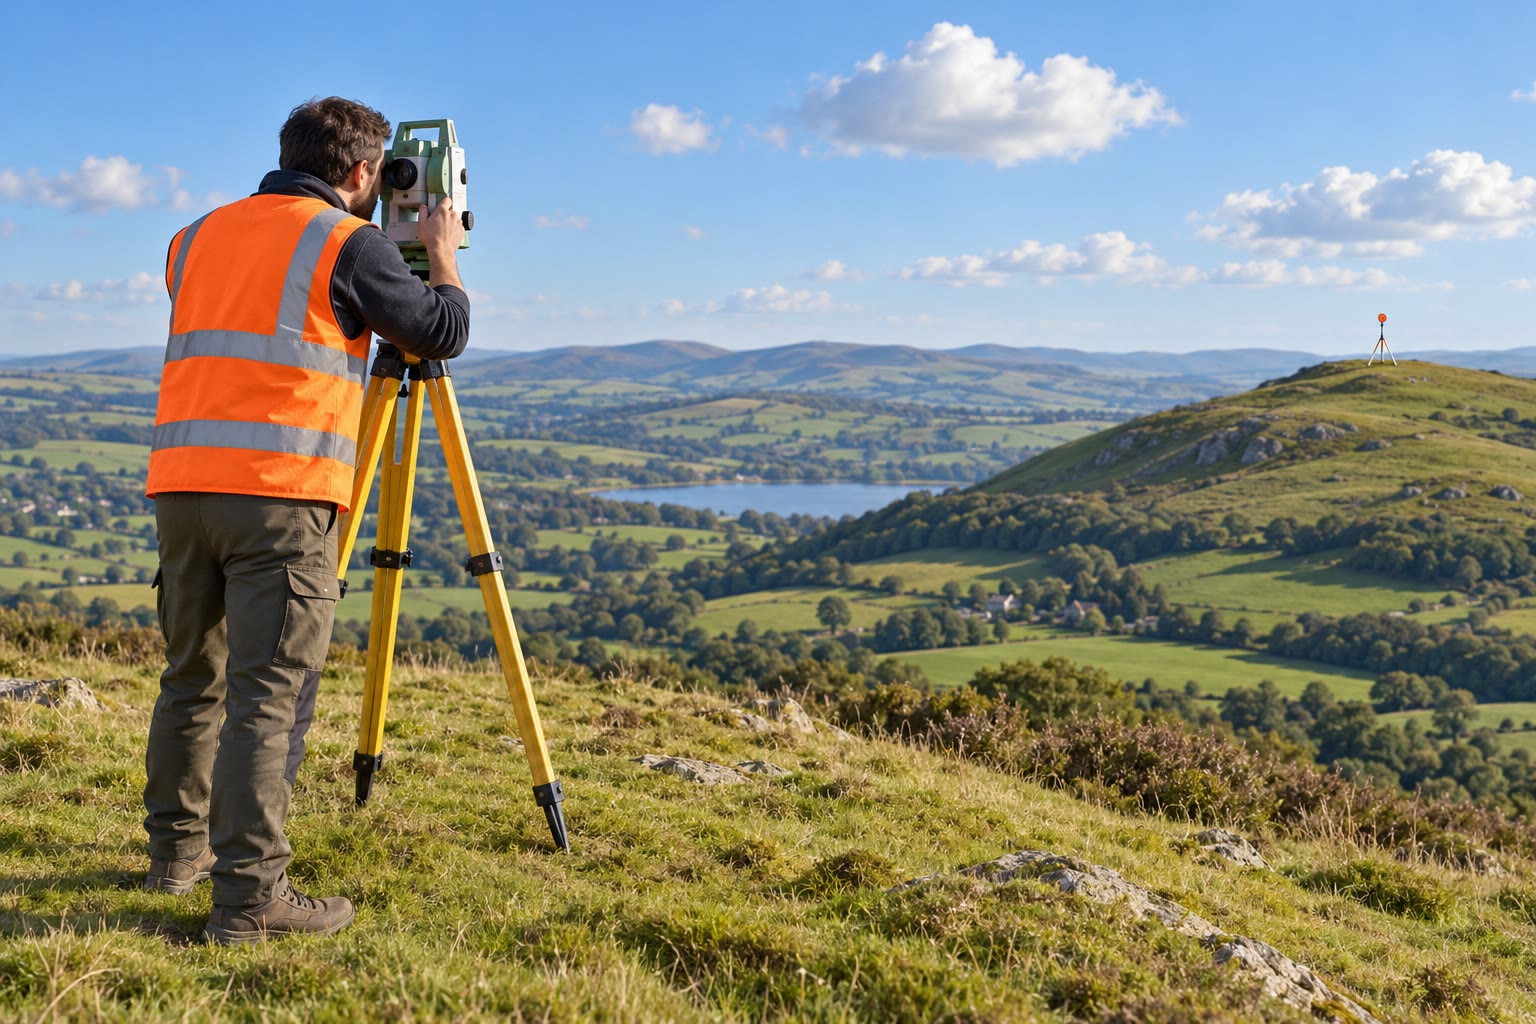
\includegraphics[width=0.7\linewidth]{images/book2/ai/g10-surveyor-theodolite.jpg}

{\small Un géomètre au travail avec un instrument moderne qui mesure les
angles et, à l'aide d'un faisceau lumineux, les distances~; un signal
géodésique se dresse sur la colline au loin.}
\end{omfigure}

Les grandes \omterm{def:g10:measuring-the-earth:triangulation}{triangulations} des \textsc{xviii}\textsuperscript{e} et
\textsc{xix}\textsuperscript{e}~siècles ont été remplacées par les
satellites. Un récepteur au sol capte les signaux de plusieurs satellites
dont la position est connue à chaque instant, et calcule sa propre position
à partir des durées de trajet des signaux (livre~1). Des réseaux de
récepteurs permanents, fixés au socle rocheux partout dans le monde,
mesurent leur position en continu. Ils définissent le système de référence
dans lequel sont données toutes les cartes et toutes les positions par
satellite, et ils bougent~: ils montrent que les plaques de la lithosphère
dérivent de quelques centimètres par an (\cref{ch:g11:plate-motions}).
% ledger: usgs:gps

\begin{inthefield}[Mesurer le sol aujourd'hui]
Les géodésiens ancrent des antennes sur des piliers de béton scellés dans
le socle rocheux, loin des bâtiments et des arbres, et enregistrent leur
position toutes les quelques secondes pendant des années. Ils combinent ces
données avec les mesures de radiotélescopes qui observent des galaxies très
lointaines et avec des faisceaux laser envoyés vers des satellites porteurs
de miroirs. Sur les chantiers et dans les campagnes, les géomètres mesurent
encore angles et distances avec des instruments sur trépied, et les
rattachent au système de référence des satellites.
\end{inthefield}

\section{Exercices}

\begin{exercise}[$\star$]\label{exo:g10:measuring-the-earth:1}
Donner trois observations, possibles sans quitter le sol, qui montrent que
la Terre est ronde. Pour chacune, expliquer en une phrase pourquoi une Terre
plate ne pourrait pas la produire.
\end{exercise}

\begin{exercise}[$\star$]\label{exo:g10:measuring-the-earth:2}
Qu'est-ce que la \omterm{def:g10:measuring-the-earth:geodesy}{géodésie}~? Qu'est-ce que la \omterm{def:g10:measuring-the-earth:triangulation}{triangulation}, et quelle est
l'unique longueur qu'il faut mesurer au sol dans une \omterm{def:g10:measuring-the-earth:triangulation}{triangulation}~?
\end{exercise}

\begin{exercise}[$\star$]\label{exo:g10:measuring-the-earth:3}
Ératosthène a trouvé que l'angle entre les rayons du Soleil et la verticale
à Alexandrie valait $1/50$ de tour complet lorsque le Soleil était au zénith
à Syène, à 5000 stades de là. Calculer la circonférence en stades, puis en
kilomètres, en prenant un stade de \qty{157.2}{m}.
\end{exercise}

\begin{exercise}[$\star$]\label{exo:g10:measuring-the-earth:4}
Un degré de latitude mesure environ \qty{111}{km}. Quelle est la longueur
d'une minute de latitude ($1/60$ de degré)~? Quelle est, à peu près, la
longueur du méridien de l'équateur au pôle~?
\end{exercise}

\begin{exercise}[$\star$]\label{exo:g10:measuring-the-earth:5}
À partir du rayon équatorial \qty{6378.137}{km} et du rayon polaire
\qty{6356.752}{km}, calculer la différence des deux rayons et
l'\omterm{def:g10:measuring-the-earth:ellipsoid}{aplatissement} $f = (a-b)/a$. Écrire $f$ sous la forme de un divisé par un
nombre entier.
\end{exercise}

\begin{exercise}[$\star\star$]\label{exo:g10:measuring-the-earth:6}
Deux villes sont situées sur le même méridien, à \qty{500}{km} l'une de
l'autre. À midi, le même jour, un bâton vertical de \qty{1.00}{m} de haut
projette une ombre de \qty{0.364}{m} dans la ville du sud et de
\qty{0.456}{m} dans la ville du nord. Calculer l'angle entre les rayons du
Soleil et la verticale dans chaque ville, puis la circonférence de la Terre.
\end{exercise}

\begin{exercise}[$\star\star$]\label{exo:g10:measuring-the-earth:7}
Dans un triangle $ABC$, la base $AB = \qty{10.00}{km}$, l'angle en $A$ vaut
\qty{62}{\degree} et l'angle en $B$ vaut \qty{71}{\degree}. Calculer
l'angle en $C$ et les longueurs $AC$ et $BC$.
\end{exercise}

\begin{exercise}[$\star\star$]\label{exo:g10:measuring-the-earth:8}
Un avion vole plein ouest le long du parallèle \qty{60}{\degree} N, de la
longitude \qty{10}{\degree} E à la longitude \qty{20}{\degree} O. En
prenant un degré de longitude de $111.3 \cos \varphi$ km, calculer la
distance parcourue. Quelle longueur aurait le même écart de longitude sur
l'équateur~?
\end{exercise}

\begin{exercise}[$\star\star$]\label{exo:g10:measuring-the-earth:9}
L'œil d'un observateur est à $h = \qty{2}{m}$ au-dessus d'une mer calme. La
ligne de visée vers l'horizon frôle la mer en $T$~; le centre de la Terre
est $O$, l'œil $E$. Expliquer pourquoi le triangle $OTE$ est rectangle en
$T$, puis utiliser le théorème de Pythagore avec $R = \qty{6371}{km}$ pour
montrer que la distance à l'horizon vaut environ $\sqrt{2Rh}$, et la
calculer.
\end{exercise}

\begin{exercise}[$\star\star$]\label{exo:g10:measuring-the-earth:10}
Lire la courbe des longueurs du degré. Entre quelles latitudes la longueur
d'un degré varie-t-elle le plus vite~? Expliquer en deux phrases pourquoi un
degré de latitude est plus long près des pôles que près de l'équateur.
\end{exercise}

\begin{exercise}[$\star\star$]\label{exo:g10:measuring-the-earth:11}
L'arc de méridien de Dunkerque à Barcelone couvre \qty{9.646}{\degree} de
latitude et mesure \qty{1072.2}{km}. Calculer la longueur moyenne d'un degré
le long de cet arc. Si tous les degrés avaient cette longueur, quelle serait
la longueur du quart de méridien~? Comparer à \qty{10002.0}{km} et
expliquer le petit écart.
\end{exercise}

\begin{exercise}[$\star\star\star$]\label{exo:g10:measuring-the-earth:12}
Ératosthène a mesuré un angle de \qty{7.2}{\degree} et une distance de 5000
stades. Si son angle avait été faux de \qty{0.1}{\degree} (trop petit), de
quel pourcentage sa circonférence aurait-elle été fausse, et dans quel
sens~? Laquelle de ses deux mesures était, selon vous, la moins précise~?
\end{exercise}

\begin{exercise}[$\star\star\star$]\label{exo:g10:measuring-the-earth:13}
Une chaîne de deux triangles~: dans $ABC$, $AB = \qty{6.000}{km}$,
$A = \qty{55}{\degree}$, $B = \qty{75}{\degree}$. Dans le triangle suivant
$ACD$, construit sur le côté $AC$, l'angle en $A$ vaut \qty{50}{\degree} et
l'angle en $C$ vaut \qty{68}{\degree}. Calculer $AC$, puis $AD$.
\end{exercise}

\begin{exercise}[$\star\star\star$]\label{exo:g10:measuring-the-earth:14}
À quelle latitude un degré de longitude est-il deux fois plus court que sur
l'équateur~? À quelle latitude est-il dix fois plus court~? Expliquer
pourquoi ces deux réponses ne dépendent pas de la taille de la Terre.
\end{exercise}

\begin{exercise}[$\star\star\star$]\label{exo:g10:measuring-the-earth:15}
Utiliser les valeurs de l'ellipsoïde~: un degré de latitude mesure
\qty{110.574}{km} à l'équateur et \qty{111.694}{km} au pôle. Sur une sphère
de même rayon moyen, un degré mesurerait \qty{111.195}{km} partout. De
combien de mètres se tromperait un géomètre qui supposerait la Terre
sphérique, sur un degré à l'équateur et sur un degré au pôle~? Pourquoi une
carte qui donne des positions au mètre près doit-elle être calculée sur
l'ellipsoïde~?
\end{exercise}

\section{Problème~: le mètre et le méridien}

\begin{problem}[{Problème du week-end --- de l'ombre d'Ératosthène à la
longueur du premier mètre}]
\label{pb:g10:measuring-the-earth:1}
% ledger: geonames:aswan, geonames:alexandria, erat:method, metre:1791, metre:survey, wgs84:ellipsoid (arc lengths and degree lengths computed in figdata/grade-10/meridian_degree.py)
Une élève refait l'histoire de la mesure de la Terre avec des nombres
modernes. Assouan, l'antique Syène, est située à la latitude
\qty{24.09}{\degree} N et Alexandrie à \qty{31.20}{\degree} N~; sur
l'ellipsoïde moderne, l'arc de méridien compris entre leurs deux parallèles
mesure \qty{788}{km}. Sur l'ellipsoïde, un degré de latitude mesure
\qty{110.57}{km} à l'équateur, \qty{111.13}{km} à \qty{45}{\degree} et
\qty{111.51}{km} à \qty{66}{\degree}, et le quart de méridien mesure
\qty{10001.966}{km}.

\medskip
\noindent\textbf{Partie I --- Ératosthène, à nouveau.}
\begin{enumerate}
  \item Calculer la différence de latitude entre Assouan et Alexandrie.
  \item Quelle fraction de tour complet représente-t-elle~? Comparer au
        $1/50$ d'Ératosthène.
  \item Calculer la circonférence de la Terre que donne la méthode
        d'Ératosthène avec ces nombres modernes.
  \item Les deux villes ne sont pas sur le même méridien~: Assouan est
        située à environ \qty{3}{\degree} de longitude à l'est d'Alexandrie.
        Quelle distance faut-il utiliser dans la méthode~: la distance en
        ligne droite entre les villes ou l'arc de méridien compris entre
        leurs parallèles~? Pourquoi~?
  \item Pourquoi faut-il mesurer les deux ombres le même jour, au midi
        local~?
\end{enumerate}

\medskip
\noindent\textbf{Partie II --- Une petite triangulation.}
On mesure une base $AB = \qty{12.000}{km}$. Depuis $A$, le signal $C$ est
vu à \qty{58}{\degree} de $B$~; depuis $B$, à \qty{66}{\degree} de $A$.
Dans le triangle suivant $ACD$, l'angle en $A$ vaut \qty{47}{\degree} et
l'angle en $C$ vaut \qty{75}{\degree}. Le côté $AD$ est orienté à
\qty{8}{\degree} à l'est du nord.
\begin{enumerate}[resume]
  \item Calculer l'angle en $C$ dans le triangle $ABC$.
  \item Calculer le côté $AC$.
  \item Calculer le côté $BC$.
  \item Calculer l'angle en $D$ dans le triangle $ACD$, puis le côté $AD$.
  \item Calculer la distance nord--sud entre $A$ et $D$.
  \item À l'aide de la longueur du degré à \qty{45}{\degree}, calculer la
        différence de latitude entre $A$ et $D$, en degrés et en minutes
        d'arc.
\end{enumerate}

\medskip
\noindent\textbf{Partie III --- Une Terre aplatie.}
\begin{enumerate}[resume]
  \item De combien de mètres un degré de latitude à \qty{66}{\degree}
        est-il plus long qu'un degré à l'équateur~?
  \item Expliquer ce que cet écart montre sur la forme de la Terre.
  \item Sur l'ellipsoïde, $a = \qty{6378.137}{km}$ et
        $b = \qty{6356.752}{km}$. Calculer $a - b$ et l'\omterm{def:g10:measuring-the-earth:ellipsoid}{aplatissement}.
  \item Expliquer pourquoi, sur une Terre aplatie, le fil à plomb en un lieu
        de latitude \qty{45}{\degree} n'est pas dirigé exactement vers le
        centre de la Terre.
\end{enumerate}

\medskip
\noindent\textbf{Partie IV --- Le premier mètre.}
\begin{enumerate}[resume]
  \item D'après la définition de 1791, quelle devrait être la longueur du
        quart de méridien, en mètres~?
  \item Le mètre en platine de 1799 a été réalisé à partir d'une valeur
        mesurée du méridien. Si le quart de méridien mesure en réalité
        \qty{10001.966}{km}, que vaut sa dix-millionième partie~?
  \item Le mètre de 1799 était-il trop long ou trop court par rapport à sa
        propre définition~? De quelle fraction~?
  \item La barre de platine reproduisait fidèlement la longueur calculée
        dans les années 1790. Le quart de méridien calculé alors était-il
        trop long ou trop court~? Expliquer.
  \item De combien de millimètres le premier mètre était-il plus court que
        la dix-millionième partie du vrai quart de méridien~? Comparer à
        l'épaisseur d'une feuille de papier, environ \qty{0.1}{mm}.
\end{enumerate}
\end{problem}
